\documentclass[a4paper, 12pt]{article}
\usepackage[left=1.5cm, text={18cm, 25cm}, top=2.5cm]{geometry}
\usepackage[utf8]{inputenc}
%\usepackage[czech]{babel}
\usepackage{cite}
\usepackage{graphicx}
\usepackage{float}
\usepackage{amsmath}
\usepackage{amsfonts}
\usepackage{amssymb}
\usepackage{mathabx}
\usepackage{stmaryrd}
\usepackage{tikz}
\usepackage{url}
\usepackage{comment}
\usepackage{listings}
\newcommand{\myuv}[1]{\quotedblbase #1\textquotedblleft}
\newcommand{\defVal}[1]{$Default=#1$}
\newcommand{\interval}[2]{\langle #1,#2 \rangle}
\newcommand{\aord}[0]{\sqsubseteq}
\newcommand{\cord}[0]{\leq}
\newcommand{\adom}[0]{Q}
\newcommand{\aitem}[0]{q}
\newcommand{\asup}[0]{\top}
\newcommand{\ainf}[0]{\perp}
\newcommand{\cdom}[0]{P}
\newcommand{\citem}[0]{p}
\newcommand{\atrans}[0]{\tau}
\newcommand{\ajoin}[0]{\circ}
\newcommand{\afun}[0]{\alpha}
\newcommand{\cfun}[0]{\gamma}
\newcommand{\wid}[0]{\triangledown}
\newcommand{\nar}[0]{\triangle}
\newcommand{\intg}[0]{\mathbb{Z}}
\newcommand{\iintg}[0]{I}
\newcommand{\ijoin}[0]{\ajoin_\iintg}

\newtheorem{exmp}{Example}[section]

\lstdefinestyle{customc}{
  belowcaptionskip=1\baselineskip,
  breaklines=true,
  frame=L,
  xleftmargin=\parindent,
  language=C,
  showstringspaces=false,
  basicstyle=\footnotesize\ttfamily,
  keywordstyle=\bfseries\color{green!40!black},
  commentstyle=\itshape\color{purple!40!black},
  identifierstyle=\color{blue},
  stringstyle=\color{orange},
}

\newtheorem{lemma}{Lemma}[section]
\newtheorem{example}{Example}[section]
\newcommand{\vata}[0]{the VATA library}
\newcommand{\Vata}[0]{The VATA library}
\newcommand{\rng}[1]{range(#1)}
\newcommand{\fagr}[0]{\otimes t_1 \cdots t_n}
\newcommand{\funcdecl}[3]{#1: #2 \rightarrow #3}
\newcommand{\subst}[2]{[#1/#2]} %co, za co
\newcommand{\bexmp}[0]{\vspace{0.2pt}\noindent\rule{\textwidth}{0.4pt}\begin{example}}
\newcommand{\eexmp}[0]{\end{example}\noindent\rule{\textwidth}{0.6pt}}
\newcommand{\symset}[0]{\mathbb{S}}
\newcommand{\instrset}[0]{\mathbb{I}}
\newcommand{\regs}[0]{\mathbb{G}}
\newcommand{\regsset}[0]{\{r_1, \ldots, r_m\}}
\newcommand{\regssub}[2]{\regs [#1 := #2]}
\newcommand{\regssubmin}[3]{\regs \setminus \{#3\} [#1 := #2]}
\newcommand{\symstate}[3]{(#1, #2, #3)}
\newcommand{\stdsym}[0]{\symstate{F}{\regs}{I}}
\newcommand{\natnum}[0]{\mathbb{N}}
\newcommand{\lang}[0]{\mathcal{L}}
\newcommand{\abp}[0]{\mathit{ABP}}
\newcommand{\glb}[0]{\mathit{GLOB}}
\newcommand{\nodelab}[0]{\mathit{NL}}
\newcommand{\rootref}[0]{\mathit{RR}}
\newcommand{\rootit}[0]{\mathit{ROOT}}
\newcommand{\displ}[0]{\mathit{DISPL}}
\newcommand{\femp}[0]{F_\mathit{Empty}}
\newcommand{\fbad}[0]{F_\mathit{BAD}}

\newcommand{\lstate}[0]{\mathit{lhs.state}}
\newcommand{\rstate}[0]{\mathit{rhs.state}}

\newcommand{\concrop}[1]{f_{\texttt{op}}(g_{#1})}

\newcommand{\defarrow}[0]{\Leftrightarrow}

\newcommand{\eqrel}[1]{\sim_#1}
\newcommand{\eqclass}[2]{[#1]_{\eqrel{#2}}}
\newcommand{\heqrel}[1]{\sim^n_#1}
\newcommand{\langlen}[2]{L^{\leq n}(#1,#2)}
\newcommand{\langstate}[2]{L(#1,#2)}
\newcommand{\heqclass}[2]{[#1]_{\heqrel{#2}}}

\newcommand{\abstr}[0]{\tau_{op}}
\newcommand{\rabstr}[0]{\tau_{-op}}
\newcommand{\abs}[0]{\alpha}
\newcommand{\pabs}[0]{\alpha_{\predset}}

\newcommand{\port}{\phi}
\newcommand{\portind}[1]{\port_{#1}}
\newcommand{\portof}[2]{\port_{#1}^{#2}}
\newcommand{\portoff}[1]{\port^{#1}}
\newcommand{\portseq}[2]{\port_{#1}^{#2} \cdots \port_{#1}^{#2}}

\newcommand{\iport}{\pi}
\newcommand{\iportof}[2]{\iport_{#1}^{#2}}
\newcommand{\iportseq}[2]{\iport_{#1}^{#2} \cdots \iport_{#1}^{#2}}

\newcommand{\fclass}[0]{\mathcal{F}}
\newcommand{\fpabs}[0]{\alpha_{\predset}^{\fclass}}

\newcommand{\pred}[0]{P}
\newcommand{\predset}[0]{\mathcal{P}}
\newcommand{\predaut}[0]{A^\mathcal{P}}
\newcommand{\predauti}[1]{A^\mathcal{P}_{#1}}
\newcommand{\peqrel}[0]{\sim_\predset}

\newcommand{\lfunc}[2]{\lambda #1 \,:\, #2}
\newcommand{\lfuncp}[3]{(\lambda #1 \,:\, #2)(#3)}

\newcommand{\ddispl}[0]{Displ}
\newcommand{\droot}[0]{Root}
\newcommand{\rref}[0]{RR=(\droot,\ddispl)}
\newcommand{\rreftuple}[2]{(#1,#2)}
\newcommand{\rrefreg}[1]{#1=(\droot,\ddispl)}
\newcommand{\ddata}[0]{D = (T,S,V,MB)}

\newcommand{\grev}[0]{g}
\newcommand{\grevinter}[0]{\symset \times \instrset \rightarrow \symset}

\newcommand{\code}[1]{\small{\texttt{#1}}}
\newcommand{\codix}[1]{\emph{\code{#1}}}

\newcommand{\sbwd}[0]{S^{B}_{i}}
\newcommand{\sbwdp}[1]{S^{B}_{#1}}
\newcommand{\isfwd}[0]{I^{F}}
\newcommand{\isfwdp}[1]{I_{#1}^{F}}
\newcommand{\sfwd}[0]{S^{F}_{i}}
\newcommand{\sfwdp}[1]{S^{F}_{#1}}
\newcommand{\ftraceseq}[0]{S^{F}_0, \ldots, S^{F}_n}
\newcommand{\ftrace}[0]{\mathit{FT}}

\newcommand{\btraceseq}[1]{S^{B}_0, \ldots, S^{B}_#1}
\newcommand{\btrace}[0]{\mathit{BT}}
%\newcommand{\isbwd}[0]{I^{B}}
\newcommand{\isbwd}[0]{I^{B}}
\newcommand{\isbwdp}[1]{I^{B}_{#1}}
\newcommand{\ipred}[0]{I_{P}}
\newcommand{\ipredb}[0]{\isbwd_{P}}
\newcommand{\bstdsym}[0]{\symstate{F}{\regs}{\isbwd}}

\newcommand{\ffwd}[0]{F^{F}}
\newcommand{\fbwd}[0]{F^{B}}


%isect
\newcommand{\A}[0]{\mathcal{A}}
\newcommand{\B}[0]{\mathcal{B}}
\newcommand{\CC}[0]{\mathcal{C}}
\newcommand{\F}[0]{\mathcal{F}}
\newcommand{\X}[0]{\mathcal{X}}
\newcommand{\nat}[0]{\mathbb{N}}
\newcommand{\st}[0]{\;|\;}
\newcommand{\ltr}[1]{\xrightarrow{#1}} % labelled->
\newcommand{\rank}[0]{\#}
\newcommand{\post}[2]{\mathit{post}_{#1}(#2)}
\newcommand{\powerset}[1]{2^{#1}}


\title{Abstract Interpretation Based On Forester Automata}
\author{Martin Hruška\\ihruska@fit.vutbr.cz}

\date{}
\begin{document}


\maketitle

\begin{abstract}
This work focuses on abstract interpretation and
forest automata and their application in shape analysis
what is a field of static analysis focuses on verification of
programs manipulating dynamic data structures.
Abstract interpretation is described as an general method
for defining semantics of programs first.
Then forest automata are introduced together with their properties
making them able to represent data structures allocated on heap.
Finally, their application in shape analysis is presented. 
\end{abstract}

\tableofcontents

\section{Introduction}
\label{sec:intro}

\emph{Abstract interpretation based on forest automata} is a technique of \emph{shape analysis}.
Shape analysis is a field of static analysis aiming to
formal verification of memory safety properties (safety properties
guarantee that nothing bad never happens) of
programs manipulating complex dynamic data structures.
The violations of the safety properties are often bugs
such as segmentation fault, invalid frees or memory leaks.
Abstract interpretation based on forest automata can detect these violations
and provide an counterexample (a particular path in analysed program
leading to a memory bug) or it can prove correctnes of program (w.r.t. given spacification)
by generation of shape invariants representing all possible shapes which
can be allocated on heap in a given point of analysed program.
When we refer to shapes of heap then it means (in context of shape analysis)
that the data structures allocated on heap are viewed
as graphs forming different shapes.
This works will firstly describe both parts, abstract interpretation and forest automata,
of the technique separately and then their
synthesis for the purposes of the analysis will be given.

Abstract interpretation is not only a method of formal verification but
it is a general framework for automatical definition or (sound) approximation of
program semantics (w.r.t. observed properties) from its source code.
The crucial component of abstract interpretation is so called
\emph{abstract domain} representing observed properties of program.
It is also necessary to model the effects of program statements
on observed properties in abstract domain.
E.g., consider an analysis of possible values of integer variables.
The concrete domain is formed by the set of integers (a set represent possible
values of a variable) and the abstract domain can be set of intervals over integers.
In such case, a concrete value $\{2,10,100\}$ of a variable could
be represented by interval $\interval{-100}{100}$ in the abstract domain.
It is of course possible to pick a more precise interval such as $\interval{2}{100}$.
A~choice of interval depends on an abstraction function
which maps values from concrete domain to abstract one.
The abstract function is often compromise between precision and computational
feasability (i.e., avoiding a state space explosion during analysis).

A~choice of abstract domain is not completly unrestricted.
The framwork of abstract interpretation requires to chose a domain
overaproximating all possible behaviours of the original program.
This means that each possible behaviour of the analysed program is included in
behaviours of the program in abstract domain.
Such overaproximation is \emph{sound} because it will not miss any
behaviour of the original program.
On the other hand, a weakness of this approaoch is \emph{incompletness}\,---\,
adding the behaviours of program not presented in the original semantics

One can ask for the reasons of the overaproximation when it leads to
imprecise information about program semantics.
The reasons are two.
The first and the main one is that the abstraction (representation in abstract domain) gives
analysis chance to terminate since the problem of defining semantics of a program is
generally undecidable (by reduction from halting problem).
The second reason is an acceleration of computation of semantics by reduction of state
space needed to explore in abstract domain in contrast to an analysis in concrete domain
which often lead to the space explosion problem and so to an exponential complexity.

The information collected by abstract interpretation can be used not only
in verification but also in automatic code optimization done by compilers
or as a support for debugging (e.g. abstract interpretation can provide data flow graph).

The other essential part of this work is forest automata (FA) theory.
Forest automata were introduced in \cite{cav11}.
They are basically tuples of tree automata (TA) (automata similiar to finite automata
but they accepts trees instead of words) which are interconnected
by references to another TA of FA in symbols from alphabet of forest automaton.
Forest automata have been designed directly for shape analysis and
they came from principles of \emph{abstract regular model checking} \cite{artmc}.
However in \cite{atva13}, they were presented as an abstract domain in abstract interpretation.
Informally, forest automata can model a certain class of data structure.
These data structures can be viewed as graphs (or shapes) that can be decomposed to the tuples
of trees (this trees are interconnected by the mentioned references).
These tuples of trees can be accepted by forest automata as the members of their languages.
Therefore forest automata can represent (by their languages) the possible shapes of heaps
and so they can be used as an abstract domain.
The abstraction techniques over forest automata were also designed
to overaproximate represented state space and makes possible for analysis to terminate.

Forest automata based abstract interpretation is done by (i) using
forest automata as an abstract domain, (ii) definition of the appropriate
operations over forest automata modelling statements in program
modifying dynamic data structures and (iii) using abstraction over FA
to enable computing all possible shapes of heap in particular
program points.
The method has ability to analyse complex dynamic data structures
such as skiplist of the second and the third level which are not
automatically analysable by any other technique.

The rest of this work is structured as follows.
In Section \ref{sec:aif}, abstract interpretation will
be formally defined and the same is done for forest automata
in Section \ref{sec:fa}.
The abstract interpretation based on forest automata is technically
described in Section \ref{sec:analysis}.

\section{Abstract Interpretation Framework}
\label{sec:aif}
We already gave some intuition about priciples of abstract interpretation in the introduction,
this sections provides with more formal and deep description of method.
First, the mentioned example about tracking integer variables is completed by
other ingrediences of abstract interpretation to deepen the intuition.
Then the formal definition of abstract interpretation is given, construction of its parts
explained and its properties described.
Finally an algorithm for computing semantics (or its overaproximation) of program
using abstract interpretation is presented.

Consider again the example of the abstract interpretation for tracking
the possible values of integer variables.
The concrete domain is a set of sets of integers $2^\mathbb{Z}$ (for simplification
we will not consider overflows of integer variables etc.).
The statements of programming language changing values of the variables
(e.g., assigment or incrementation) are called \emph{concrete transformers}.
A~concrete analysis over the concrete domain with the conrete transformers
would led to non-termination of analysis because infinite space may arise.
The non-termination problem can be addressed by doing the analysis in abstract domain.
The abstract domain is a set of intervals over $\mathbb{Z}$.

To model the semantics of program in abstract domain, it is necessary to define
abstract transformers modelling the concrete semantics.
The abstract transformers should reflect an effect of a concrete transformer
on the properties tracked by abstract interpretation.
In our example, consider the variables $x$ and $y$ assigned values $(-\infty,-100\rangle$
and $(-100, 100)$ in abstract domain.
The abstract transformer corresponding to arithmetic addition $+$
should for $x+y$ give the result $(-\infty,100)$.

Moreover, we will need to define operator joining possible values
of a variable over more paths in program.
The examples of program points, where such an operator is needed, is
the end of \texttt{if} statement or the beginning of \texttt{while} loop.
E.g., the join of a variable $x$
with the abstract value $\interval{100}{200}$ in \texttt{then} branch
of if statement and $\interval{400}{500}$ in \texttt{else} branch
would result to the abstract value $\interval{100}{500}$ taking the smaller beginning
and greater end of the both intervals as the boundaries of the new interval.

The join operator should result to the greater or
equal abstract value compared to the inputs of the operator.
This is key property of join operator.
An ordering $\aord$ over the values in abstract domain is therefore needed
to enable checking of this property of join operator.

Now we will continue from the intuitive description to
the formal definition of abstract interpretation (definitions
are given in the same way as in \cite{popl77}).

\subsection{Formal Definition of Abstract Interpretation}
\emph{Abstract Interpretation} $I$ of a program $P$ is a tuple
$I=(\adom, \ajoin, \aord, \asup, \ainf, \atrans)$ where
\begin{itemize}
	\item $\adom$ is an abstract domain
	\item $\ajoin: \adom \times \adom \rightarrow \adom$ is a join operator
	\item $\aord \subseteq \adom \times \adom$ is a relation (ordering) such that $\forall x,y \in \adom: x \aord y \leftrightarrow x \ajoin y = y$
	\item $\asup$ is a supremum of $\adom$
	\item $\ainf$ is a infinum of $\adom$
	\item $\atrans = \{\adom \times \ldots \times \adom \rightarrow \adom\}$ is a set of abstract transformers, where a length of
		the sequence $\adom \times \ldots \times \adom$ determines arity of abstract transformer
\end{itemize}


$(\adom, \ajoin, \aord, \top, \perp)$ forms a complete semilattice.

Abstract transformers can be specified by formalization of behaviour of concrete instructions
of program using e.g., denotational or operational semantics w.r.t. properties tracked
by abstract interpretation.
Therefore when a programming language has a well-defined semantics then
it is possible to use abstract interpretation as a method for computation
of a program written in this programming language.

The most important characteristics of abstract interpretation
are going to be described in the following section.
Since abstract interpretation overaproximates possible behaviours of
the concrete system it is a \textbf{sound} method.
A~prove of soudness will be informally described using
two auxiliary functions $\afun, \cfun$ for switching between abstract and concrete domain.
An abstraction function $\afun: \cdom \rightarrow \adom$ assigns to an item from
concrete domain an item form abstract domain and a concretization function
$\cfun: \adom \rightarrow \cdom$ maps values from abstract domain back to concrete domain.
Assume also an ordering $\cord \subseteq \cdom \times \cdom$.
Triples $(\adom, \aord, \afun)$ and $(\cdom, \cord, \cfun)$ form
\emph{Gallois connections} \cite{popl77} which is defined as follows:
\begin{center}
	$(\adom, \aord, \afun, \cfun, \cord, \cdom)$ is Gallois connections iff
	$(\adom, \aord)$ and $(\cdom, \cord)$ are posets and
	$\forall \citem \in \cdom \, \forall \aitem \in \adom: \citem \cord \cfun(\aitem)
	\Leftrightarrow \aitem \aord \afun(\citem)$
\end{center}

The properties of Gallois connections implies that
$\forall \citem \in \cdom: \citem \cord \cfun(\afun(\citem))$.
Let $q = \afun(\citem)$ then it holds $\alpha(\citem) \aord \aitem$,
thus $\citem \cord \cfun(\aitem)$ and finally $\citem \cord \cfun(\afun(\citem))$.
We get that a concretization of an abstracted configuration of concrete system
is greater than the original value and covers the original configuration.
Another necessary property of abstract interpretation leading to soudness is
that abstract transformers do not violate Gallois connection.
Formally, $\alpha(I(\citem_1,\ldots,\citem_n)) \cord \atrans_I(\alpha(\citem_1),\ldots, \alpha(\citem_n))$
where $\citem_1,\ldots,\citem_n \in \cdom$ and $\atrans_I$ is an abstract transformer
modelling semantics of an instruction $I$ in concrete program.
These two properties of abstract domain and abstract transfomers ensures
soundness of abstract interpretation.

On the other hand, abstract interpretation is not \textbf{complete}.
The fact $\citem \cord \cfun(\afun(\citem))$ (a concretization of abstracted value
is something greater) implies that an abstraction of concrete value may lead
to overaproximation of possible behaviours.
This is undesirable in the applications such as formal verification
where the behaviours added by overaproximation can contain
a violation of the checked properties.

A~possible solution of problems caused by incompletness is a refinement of the abstraction.
However, an immoderate refinement can led to infeasable computational complexity
or even to nontermination of the method.
Generally, \textbf{termination} of abstract interpretation is guaranteed
when abstract domain $\adom$ satisfies that Kleene's sequence is finite \cite{popl77}.
This is achieved when abstract domain is finite, a length of any strictly
increasing chain is finite, or abstract domain satisfies the ascending chain
condition (every strictly increasing chain is finite, although not bounded).
Then the termination comes from Kleene's fixpoint theorem.
When abstract domain contains infinite Kleene's sequence then
then the abstract transformers can be chosen to allow only finite
Kleene's sequences during abstraction.
When the abstract domain has infinite Kleene's sequences and
the abstract transformers do not exclude them from computation during abstract
interpretation then the sequences should be truncated or computation
of fixpoint approximated by some heuristic.
Finally, when only the finite Kleene's sequences occur then
the termination of the method is guaranteed by Kleene's fixpoint theorem.

The abstraction brings inherently certain trade-off between
precision and efficiency of the method.
When the abstraction is very precise then the analysis
is slower because larger state space has to be explored.

In abstract interpretation, the mentioned approximation of fixpoint is
used in computation of all possible behaviours of for a givem program point.
The approximation is primarly necessary in the loop points of
progam where a new possible behaviour of a program can be generated
in each loop cycle.
This could lead to unbounded sequence of possible behaviours and
nontermination of the analysis.
A~concept of \emph{widening} is introduced to resolve such cases.
The~binary operation $\wid: \adom \times \adom \rightarrow \adom$ is widening iff:
\begin{itemize}
	\item $\forall \aitem, \aitem' \in \adom: \aitem \ajoin \aitem' \aord \aitem \wid \aitem'$
	\item Every infinite sequence $s_0, \ldots, s_i, \ldots$ such that
		$s_0 = C_0$ and $s_i = s_{i-1} \wid C_i$, where $C_0, C_i \in \adom$,
		is not strictly increasing.
\end{itemize}

Informally, using widening $\wid$ instead of join $\ajoin$ is one of possible heuristic
which will approximate fixpoint infinite Kleene's sequence.
It also accelerates the fixpoint computation compared with join because
$\forall \aitem, \aitem' \in \adom: \aitem \ajoin \aitem' \aord \aitem \wid \aitem'$.

The opposite operation to widening is \emph{narrowing}.
While widening accelerates computation narrowing
refines the overaproximation to get a more precise information.
Formally, the binary operation $\nar: \adom \times \adom \rightarrow \adom$
is widening iff:
\begin{itemize}
	\item $\forall \aitem, \aitem' \in \adom: (\aitem' \aord \aitem) \Rightarrow \aitem' \aord \aitem \nar \aitem' \aord \aitem$
	\item Every infinite sequence $s_0, \ldots, s_i, \ldots$ such that
		$s_0 = C_0$ and $s_i = s_{i-1} \nar C_i$, where $C_0, C_i \in \adom$,
		is not strictly decreasing.
\end{itemize}

Although the widening refines the abstraction it does not
break conditions guaranteeing fixpoint computation or approximation
what comes from the second point of widening definition.

We defined abstact interpretation and its basic properties
but we have not mentioned how to use it for computing
semantics of program.
Consider a program $P$ with program points denoted $P_i$
where $i$ is an index of a program location.
We set the initial values of the tracked semantics properties
to $\ainf$ for each program point $i$.
Then the corresponding abstract transformers in the given program point
are applied repetatively until a fixpoint in each location is reached.
The changes in tracked values in one program locations are propagated to each
iteration to the subsequent locations.
Join, widening (and if needed also narrowing) is applied at the program points
where more paths such as loop points or ends of conditions meet.
The abstract transformers are applied using round robin algorithm where
the order of transformers is defined by the original program locations.

Another possible point of view to the computation of semantics of a program using
abstract interpretation is a system of equitation.
Each program location with its dedicated abstract transformer can be viewed
as one equtiation.
The different equitations share variables what leads to propagation
of values between equitation.
An existence of (aproximate) solution of this system of equitations
is guaranteed by existence fixpoint for computation by abstract interpretation.

While the firest mentioned approach to computing the semantics of a program is
closer to implementation perspective, the second one is often used in papers
focusing on theoretical aspects of abstract interpretation and
the related mathematical background.
\newpage

\bexmp
The example about tracking integer values will be completed
in notion of the defined framework.
The example is taken from \cite{popl77}.
We want to instantiate abstract interpretation framework for aproximating
possible values of integer variables in given program location.
Conrete domain is $2^\mathbb{\intg}$, so each variable
has a value from a set from $2^\mathbb{\intg}$ which it can
gain in given program location.

The abstract interpretation is $(\iintg, \ijoin, \interval{-\infty}{\infty}, \interval{}{}, \atrans)$ where 
\begin{itemize}
	\item $\iintg = \{\interval{x}{y} \,|\, x,y \in \intg \wedge x \leq y\}$
	\item $\interval{x}{x'}, \interval{y}{y'} \in \iintg: \interval{x}{x'} \ijoin \interval{y}{y'}
		= \interval{min(x,y)}{max(x',y')}$. Informally, $\ijoin$ is a union of two intervals
	\item $\interval{}{}$ is an empty interval
	\item $\atrans$ will be defined on demand for instructions used in the following example program
\end{itemize}

Consider the following program in the $C$ language, where $C_i$ in a comment is labeling
of a particular program point $i$.

\lstinputlisting[caption=Example program, style=customc]{example.c}

The only integer variable in program is $x$. As the next step,
the system of equitations for the program will be assembled
to compute the possible abstract values of $x$ in each program point.
But first we have to define the following two operators:
\begin{itemize}
	\item $+: \interval{x}{x'} + \interval{y}{y'} = \interval{x+y}{x'+y'}$
	\item $\cap: \interval{x}{x'} \cap \interval{y}{y'} = \interval{max(x,y)}{min(x,y)}$
\end{itemize}

The equitations are following:
\begin{enumerate}
	\item $C_0 = \interval{}{}$
	\item $C_1 = \interval{1}{1}$
	\item $C_2 = C_1 \ijoin C_4$
	\item $C_3 = C_2 \cap \interval{-\infty}{100}$
	\item $C_4 = C_3 + \interval{1}{1}$
	\item $C_5 = C_2 \cap \interval{101}{\infty}$
\end{enumerate}

The semantics of $C_1 = \interval{1}{1}$ is that the variable $x$ has a value from interval $\interval{1}{1}$
at the program point $C_1$. The semantics of the other equitations are analogical.

If we start computation of fixpoint using just $\ijoin$ operator the computation takes $101$ steps
before the fixpoint is reached.
That is maximal number of iteration of the \texttt{while} cycle.
The possitive message is that the computation will terminate, the negative one
is that it will take quite a long time for such a simple program.
Therefore we introduce widening $\wid$ defined as follows:
\begin{itemize}
	\item $\interval{}{}$ is the null element of $\wid$
	\item $\interval{x}{x'} \wid \interval{y}{y'} = \interval{(x < y)\,?\,-\infty\,:\,x}{(y' > x')\,?\,\infty\,:\,x'}$
\end{itemize}
where $?:$ is a ternary operator with the same semantics as in the $C$ language.

The equitation $3$ will be modified using the widening:
$C_2 = C_2 \wid (C_1 \ijoin C_4)$.

The approximation of solution is computed in the following iterations:
\begin{enumerate}
	\setcounter{enumi}{-1}
	\item \hspace{-0.5em} iteration:
		\begin{itemize}
			\item $\forall i \in \{0,\ldots,5\}: C_i = \interval{}{}$
		\end{itemize}
	
	\item \hspace{-0.5em} iteration:
		\begin{itemize}
			\item $C_1 = \interval{1}{1}$
			\item $C_2 = \interval{1}{1}$
			\item $C_3 = \interval{1}{1}$
			\item $C_4 = \interval{2}{2}$
		\end{itemize}
	
	\item \hspace{-0.5em} iteration:
		\begin{itemize}
			\item $C_2 = \interval{1}{1} \wid (\interval{1}{1} \ijoin \interval{2}{2})
		               = \interval{1}{1} \wid \interval{1}{2} = \interval{1}{\infty}$
			\item $C_3 = \interval{1}{100}$
			\item $C_4 = \interval{2}{101}$
			\item $C_5 = \interval{101}{\inf}$
		\end{itemize}
\end{enumerate}

Another iteration would not change anything so the fixpoint is reached.
The widening operator definitely accelerated the computation and
saved $98$ iterations.
On the other hand, the information about values at points in $C_2$ and $C_5$
is very rough due to abstraction.

The loss of information can be reduced by narrowing operator $\nar$ with
this definition:
\begin{itemize}
	\item $\interval{}{}$ is the null element of $\nar$
	\item $\interval{x}{x'} \nar \interval{y}{y'} =
		\interval{(x == -\infty)\,?\,y : min(x,y)}{(x' == \infty)\,?\,y' : max(x',y')}$
\end{itemize}

We update $2.$ equtation using narrowing:
$C_2 = C_2 \nar (C_1 \ijoin C_4)$.
The computed solution of equitations will be refined in the following iterations:
\begin{enumerate}
	\setcounter{enumi}{2}
	\item \hspace{-0.5em} iteration:
		\begin{itemize}
			\item $C_2 = C_2 \nar (C_1 \ijoin C_4) = \interval{1}{\infty} \nar
				(\interval{1}{1} \ijoin \interval{2}{101}) = \interval{1}{\infty} \nar \interval{1}{101} = 
				\interval{1}{101}$
			\item $C_3 = \interval{1}{101} \cap \interval{-\infty}{100} = \interval{1}{100}$
			\item $C_5 = \interval{1}{101} \cap \interval{101}{\infty} = \interval{101}{101}$
		\end{itemize}
\end{enumerate}

After the narrowing the information is much more precise and only one iteration
was needed so $97$ iterations were saved compared to the computation without
widening and narrowing.

Another advantage of analysis of the program in abstract domain is a compact
representation using intervals instead of set of integer values in concrete domain.
Moreover, the used abstraction (narrowing operator) would not be possible in
concrete domain because we are not able to work with an infinite set.
\eexmp


As we mentioned, the framework of abstract interpretation is general and
the preceding example is just a special case.
Many other static analysis can be formulated as
an abstract interpretation, e.g., data flow analysis,
pointer analysis, or correct array access analysis.

\section{Forest Automata}
\label{sec:fa}

This section gives an introduction to forest automata.
First the definition of the tress and graphs are given.
Then the automata accepting them are defined.
The goal is to introduce the automata in a general way
but we will aim mainly to the aspects needed for abstract interpretation.

\subsection{Graphs, Trees and Forests}
\label{sec:graph}

In the following text we use $dom(f)$ to denote a domain of a total mapping $\funcdecl{f}{A}{B}$.
The range of such mapping is denoted by $\rng{f}$.
A~symbol $a_i$ is the $i$-th symbol of a word $w = a_1 \cdots a_n$ over an alphabet $\Sigma$.

\subsubsection{Graphs and Trees}
\label{subsec:graph}
We need for purposes of graphs introduce a \emph{ranked alphabet}.
Intuitively, it is an alphabet which symbols have an integer rank.
When a symbol with a given rank $n$ appears in a labelled graph
then it is required for a symbol to be over exactly $n$ edges
leading from one node to $n$ successors.
Formally, a~\emph{ranked alphabet} is a finite set of symbols $\Sigma$
and a related mapping $\funcdecl{\#}{\Sigma}{\mathbb{N}}$ assigning to a symbol its rank.
A~(directed, ordered, labelled) \emph{graph} is a total map $\funcdecl{g}{V}{\Sigma \times V^{*}}$ where $V$ is a finite set of nodes.
We call the symbols from $\Sigma$ \emph{labels} in context of the graphs.
The map $g$ maps each node $v\in V$ to:
\begin{enumerate}
	\item a label $\alpha \in \Sigma$ that we denote by $l_g(v)$,
	\item a sequence of \emph{successors} $(v_1 \cdots v_n) \in V^n$ for $n \in \mathbb{N}$.
		We denote successors by $S_g(v)$ and $v_i$ is denoted by $S^i_g(v)$.
	\item symbol $l_g(v)$ is such that $\#(l_g(v)) = |S_g(v)|$.
\end{enumerate}

A~pair $v \mapsto (a, v_1 \cdots v_n)$ where $v, v_1, \ldots, v_n \in V$,
$a \in \Sigma$ such that $g(v) = (a, v_1 \cdots v_n)$, is called an \emph{edge} of $g$.
A~\emph{leaf} of $g$ is a node $v \in V$ without successor so it holds $S_g(v) = \epsilon$.
Consider set of all sequences of successors in which a node $v' \in V$ appears, then
the cardinality of this set is the \emph{in-degree} of a node $v' \in V$ (denoted by $idg_g(v')$).
More intuitively, the in-degree of a node is a number of the incoming edges to the node.
Formally, in-degree is defined as
$idg(v') = |\{(v \mapsto (a, v_1 \cdots v_n),i)) \,|\, v~\mapsto (a, v_1 \cdots v_n)
\text{ is an edge such that } i \in \{1,\ldots,n\}: v' = v_i\}|$.
When a node $v' \in V$ has $idg(v') > 1$ it is called a \emph{join}.

A~special case of a graph is a~\emph{tree}.
Informally, a tree is a graph which each node is
a~successor of at most one of the other nodes.
The node which is not a successor of any node is called \emph{root}.
Formally, $t$ is a graph which is either empty, or it has exactly one root and $\forall v~\in V: idg(v) \leq 1$ (informally,
each node is a successor of at most one of the other nodes).

A~\emph{path} from $v\in V$ to $v' \in V$ is a sequence $p=v_0, i_1, v_1, \ldots, i_n, v_n$ where $v=v_0, v' = v_n$
and $\forall j \in \{1,\ldots,n\}: v_j = S^{i_j}(v_{j-1})$ ($v_j$ is the $i_j$-th successor of $v_{j-1}$).
The~\emph{length} of the path $p$ is $n$ what is denoted by $length(p) = n$.
The~path $p=v_0,i_1,v_1,\ldots,i_n,v_n$ is acyclic if $\forall v_i,v_j \in p: i \neq j \Rightarrow v_i \neq v_j$.
The~\emph{cost} of the acyclic path $p$ is the sequence $i_1, \ldots, i_n$.
The~path $p$ is \emph{cheaper} than path $p'$ iff the cost of $p$ is lexicographically smaller than that of $p'$. 
A~node $u \in V$ is \emph{reachable} from a node $v \in V$ iff there exists a path from $v$ to $u$ or $u=v$.
A~node $u \in V$ is a \emph{root} of the graph $g$ iff all nodes $v \in V$ are reachable from $u$
and $u$ is not successor of any other state.
We alternatively define a root of a graph by a mapping $\funcdecl{root}{g}{V}$
which maps a graph to its root.

An example of a graph with $V=\{v_1,v_2,v_3,v_4,v_5\}$ and
the alphabet $\Sigma = \{a,b\}$ with~a ranking function $\#$ such that $\#(a) = 2$ and $\#(b) = 0$
is in Figure \ref{fig:graph_tree}.
This graph is also a tree.

	\begin{figure}[bth]
		\begin{center}
			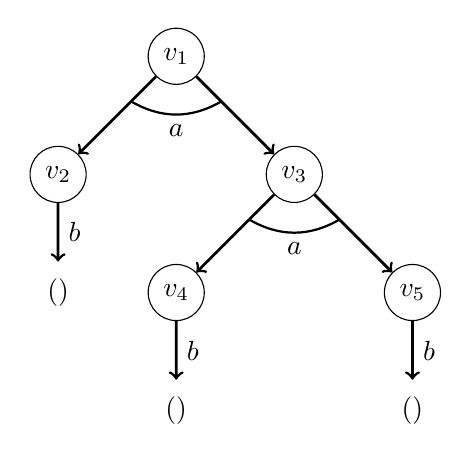
\begin{tikzpicture}[
  scale=0.8,
  node distance = 1.5cm,
  tnode/.style={circle, text centered, draw=black},
  lnode/.style={circle, text centered},
  arw/.style={->, line width=1pt},
  symline/.style={-, line width=0.8pt}
  ]

\node [tnode] (v1) {$v_1$};
\node [tnode, left of=v1, below of=v1] (v2) {$v_2$};
\node [left of=v1, below of=v1, above of=v2, right of=v2, yshift=1cm, xshift=0.8cm] (v1v2) {};
\node [tnode, right of=v1, below of=v1] (v3) {$v_3$};
\node [left of=v1, below of=v1, above of=v3, right of=v3, yshift=1cm, xshift=-0.8cm] (v1v3) {};
\node [lnode, below of=v2] (v02) {$()$};

\node [tnode, below of=v3, left of=v3] (v4) {$v_4$};
\node [left of=v3, below of=v3, above of=v4, right of=v4, yshift=1cm, xshift=0.8cm] (v3v4) {};
\node [tnode, below of=v3, right of=v3] (v5) {$v_5$};
\node [left of=v3, below of=v3, above of=v5, right of=v5, yshift=1cm, xshift=-0.8cm] (v3v5) {};
\node [lnode, below of=v4] (v04) {$()$};
\node [lnode, below of=v5] (v05) {$()$};

\draw [arw] (v1) -- (v2);
\draw [arw] (v1) -- (v3);
\draw [arw] (v2) -- node [midway, right] {$b$} (v02);
\draw [arw] (v3) -- (v4);
\draw [arw] (v3) -- (v5);
\draw [arw] (v4) -- node [midway, right] {$b$} (v04);
\draw [arw] (v5) -- node [midway, right] {$b$} (v05);

\draw [symline] (v1v2) edge [bend right] node [midway, below] {$a$} (v1v3);
\draw [symline] (v3v4) edge [bend right] node [midway, below] {$a$} (v3v5);

\end{tikzpicture}

		\end{center}
		\caption{A~graph $t$ that has attributes of a tree.}
		\label{fig:graph_tree}
	\end{figure}
	\label{ex:graph}

\subsubsection{Forests}
\label{subsec:forests}

In this section we assume without the loss of generality that $\Sigma \cap \mathbb{N} = \emptyset$.
A~$\Sigma$-labelled \emph{forest} is a sequence of trees $t_1 \cdots t_n$ over ($\Sigma \cup \{1,\ldots,n\}$)
where $\forall i \in \{1,\ldots,n\}: \#i = 0$ (the rank of new symbols from $\mathbb{N}$ is zero).
We suppose that the sets of nodes of the trees $t_1, \ldots, t_n$ are disjoint.
\emph{Root references} are leaves labelled by a label $i \in \{1,\ldots,n\}$.
The newly added symbols from $\{1,\ldots,n\}$ labelling root references are
supposed to interconnect trees in a forest.
E.g., when the second tree has a leaf $v$ which is a root reference labelled by $1$
then it is symbolical connection of the leaf $v$ of the second tree
with the root of the first tree.
The forest $t_1 \cdots t_n$ represents the graph $\fagr$ that arises
by interconnecting roots by the related root reference.
Formally, the graph $\fagr$ contains an edge $v \mapsto (a,v_1 \cdots v_m)$ iff $\exists i \in \{1, \ldots, n\}:\ \exists(v \mapsto (a, v_1' \cdots v_m')) \in edges(t_i):
\ \forall j \in \{1,\ldots,m\}: v_j = h(v_j')$ where $edges(t_i)$ is the set of all edges of the tree $t_i$ and
\[ h(v_j') = \left\{
  \begin{array}{l l}
  root(t_k) & \quad \text{if $v_j'$ is a root reference with $l(v_j') = k$}\\
  v_j'   & \quad \text{otherwise.}
  \end{array} \right.\]

Consider a forest $f$ over $\Sigma \cup \{\overline{2}, \overline{3}\}$
($\Sigma$ is the same one as in Figure \ref{ex:graph}) in Figure \ref{fig:forest}.
The graph $\otimes t_1,t_2,t_3$ obtained by interconnecting trees in the forest $f$ is in Figure \ref{fig:forest_graph}.

	\begin{figure}[bth]
	\begin{center}
		\scalebox{1}
		{
			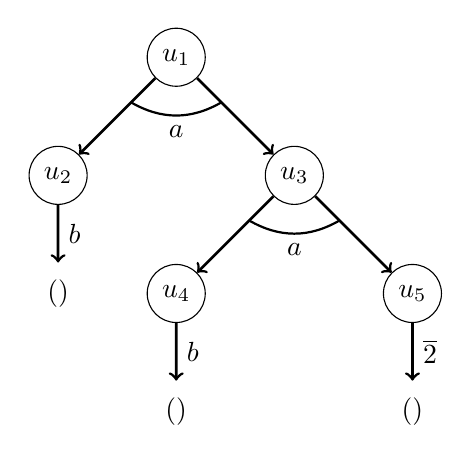
\begin{tikzpicture}[
  scale=0.8,
  node distance = 1.5cm,
  tnode/.style={circle, text centered, draw=black},
  lnode/.style={circle, text centered},
  arw/.style={->, line width=1pt},
  symline/.style={-, line width=0.8pt}
  ]

\node [tnode] (u1) {$u_1$};
\node [tnode, left of=u1, below of=u1] (u2) {$u_2$};
\node [left of=u1, below of=u1, above of=u2, right of=u2, yshift=1cm, xshift=0.8cm] (u1u2) {};
\node [tnode, right of=u1, below of=u1] (u3) {$u_3$};
\node [left of=u1, below of=u1, above of=u3, right of=u3, yshift=1cm, xshift=-0.8cm] (u1u3) {};
\node [lnode, below of=u2] (u02) {$()$};

\node [tnode, below of=u3, left of=u3] (u4) {$u_4$};
\node [left of=u3, below of=u3, above of=u4, right of=u4, yshift=1cm, xshift=0.8cm] (u3u4) {};
\node [tnode, below of=u3, right of=u3] (u5) {$u_5$};
\node [left of=u3, below of=u3, above of=u5, right of=u5, yshift=1cm, xshift=-0.8cm] (u3u5) {};
\node [lnode, below of=u4] (u04) {$()$};
\node [lnode, below of=u5] (u05) {$()$};

\draw [arw] (u1) -- (u2);
\draw [arw] (u1) -- (u3);
\draw [arw] (u2) -- node [midway, right] {$b$} (u02);
\draw [arw] (u3) -- (u4);
\draw [arw] (u3) -- (u5);
\draw [arw] (u4) -- node [midway, right] {$b$} (u04);
\draw [arw] (u5) -- node [midway, right] {$\overline{2}$} (u05);

\draw [symline] (u1u2) edge [bend right] node [midway, below] {$a$} (u1u3);
\draw [symline] (u3u4) edge [bend right] node [midway, below] {$a$} (u3u5);

\end{tikzpicture}

			\hspace{0.55cm}
			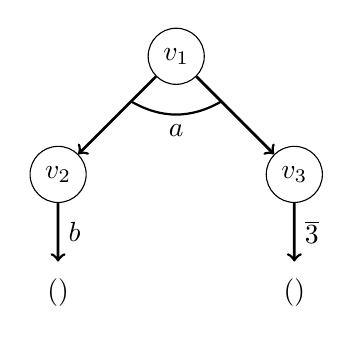
\begin{tikzpicture}[
  scale=0.8,
  node distance = 1.5cm,
  tnode/.style={circle, text centered, draw=black},
  lnode/.style={circle, text centered},
  arw/.style={->, line width=1pt},
  symline/.style={-, line width=0.8pt}
  ]

\node [tnode] (v1) {$v_1$};
\node [tnode, left of=v1, below of=v1] (v2) {$v_2$};
\node [left of=v1, below of=v1, above of=v2, right of=v2, yshift=1cm, xshift=0.8cm] (v1v2) {};
\node [tnode, right of=v1, below of=v1] (v3) {$v_3$};
\node [left of=v1, below of=v1, above of=v3, right of=v3, yshift=1cm, xshift=-0.8cm] (v1v3) {};
\node [lnode, below of=v2] (v02) {$()$};
\node [lnode, below of=v3] (v03) {$()$};

\draw [arw] (v1) -- (v2);
\draw [arw] (v1) -- (v3);
\draw [arw] (v2) -- node [midway, right] {$b$} (v02);
\draw [arw] (v3) -- node [midway, right] {$\overline{3}$} (v03);

\draw [symline] (v1v2) edge [bend right] node [midway, below] {$a$} (v1v3);

\end{tikzpicture}

			\hspace{0.55cm}
			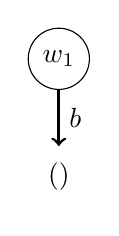
\begin{tikzpicture}[
  scale=0.8,
  node distance = 1.5cm,
  tnode/.style={circle, text centered, draw=black},
  lnode/.style={circle, text centered},
  arw/.style={->, line width=1pt},
  symline/.style={-, line width=0.8pt}
  ]

\node [tnode] (w1) {$w_1$};
\node [lnode, below of=w1] (w01) {$()$};

\draw [arw] (w1) -- node [midway, right] {$b$} (w01);

\end{tikzpicture}

		}
		\caption{A~forest $f$ consisting 3 trees $t_1, t_2, t_3$ with roots $u_1, v_1, w_1$.}
	  \label{fig:forest}
	\end{center}
	\end{figure}

	\begin{figure}[bth]
	\begin{center}
		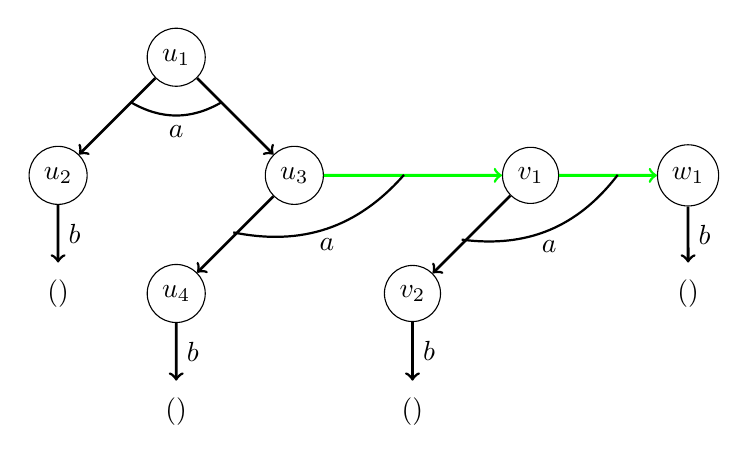
\begin{tikzpicture}[
  scale=0.8,
  node distance = 1.5cm,
  tnode/.style={circle, text centered, draw=black},
  lnode/.style={circle, text centered},
  arw/.style={->, line width=1pt},
  symline/.style={-, line width=0.8pt}
  ]

% tree 1

\node [tnode] (u1) {$u_1$};
\node [tnode, left of=u1, below of=u1] (u2) {$u_2$};
\node [left of=u1, below of=u1, above of=u2, right of=u2, yshift=1cm, xshift=0.8cm] (u1u2) {};
\node [tnode, right of=u1, below of=u1] (u3) {$u_3$};
\node [left of=u1, below of=u1, above of=u3, right of=u3, yshift=1cm, xshift=-0.8cm] (u1u3) {};
\node [lnode, below of=u2] (u02) {$()$};

\node [tnode, below of=u3, left of=u3] (u4) {$u_4$};
\node [left of=u3, below of=u3, above of=u4, right of=u4, yshift=0.8cm, xshift=0.6cm] (u3u4) {};
\node [lnode, below of=u4] (u04) {$()$};

\node [right of=u3, left of=v1, right of=u1, below of=u1, xshift=1.5cm, yshift=0.13cm] (u3v1) {};

\draw [arw] (u1) -- (u2);
\draw [arw] (u1) -- (u3);
\draw [arw] (u2) -- node [midway, right] {$b$} (u02);
\draw [arw] (u3) -- (u4);
\draw [arw] (u4) -- node [midway, right] {$b$} (u04);

\draw [symline] (u1u2) edge [bend right] node [midway, below] {$a$} (u1u3);

% tree 2
\node [tnode, right of=u1, right of=u3] (v1) {$v_1$};
\node [tnode, left of=v1, below of=v1] (v2) {$v_2$};
\node [left of=v1, below of=v1, above of=v2, right of=v2, yshift=0.7cm, xshift=0.5cm] (v1v2) {};
\node [lnode, below of=v2] (v02) {$()$};

\draw [arw] (v1) -- (v2);
\draw [arw] (v2) -- node [midway, right] {$b$} (v02);

%tree 3
\node [tnode, right of=v1, xshift=0.5cm] (w1) {$w_1$};
\node [lnode, below of=w1] (w01) {$()$};
\node [right of=v1, left of=w1, yshift=0.13cm, xshift=-0.8cm] (v1v3) {};

\draw [arw] (w1) -- node [midway, right] {$b$} (w01);

%\draw [arw] (w1) -- node [midway, right] {$b$} (w01);

%connection

\draw [arw, color=green] (u3) -- (v1);
\draw [arw, color=green] (v1) -- (w1);

\draw [symline] (u3u4) edge [bend right] node [midway, below] {$a$} (u3v1);
\draw [symline] (v1v2) edge [bend right] node [midway, below] {$a$} (v1v3);

\end{tikzpicture}

		\caption{The graph $\otimes t_1,t_2,t_3$ obtained from the forest $f$ in Figure \ref{fig:forest}.
		The green edges are the ones that were added to create the graph from the forest $f$.}
	  \label{fig:forest_graph}
	\end{center}
	\end{figure}
\vspace{-0.5cm}

\subsubsection{Graphs and Forests with Ports}
\label{subsec:gfp}

We mark some graph node as \emph{input} or \emph{output} one what is later needed for manipulation
with forest automata of higher degree.
The marking of input and output port is done by tuple of so-called \emph{ports} in the following way.
An \emph{input-output-graph} (io-graph) is a pair $(g,\phi)$ (also denoted by $g_\phi$)
where $g$ is a graph and $\phi=(\phi_1 \cdots \phi_n) \in dom(g)^+$ is a sequence of ports,
where $\phi_1$ is the input port and $\phi_2 \cdots \phi_n$ are output ports.
The ports are unique in $\phi$.
The graph $g_\phi$ is called \emph{accessible} if its root is the input port $\phi_1$.

The \emph{cut-points} $cps(g_\phi)$ of a graph $g_\phi$ are ports and joins of the graph,
i.e. $cps(g_\phi)=\{v \in V\,|\, v~\in \phi \vee idg(v) > 1\}$.

An \emph{io-forest} is straightforward extension of a forest with concept of input and output ports.
We add a sequence of numbers which denote the trees of the forest whose roots would
be input and output of an interconnected graph of the io-forest.
Formally, an \emph{io-forest} is a pair $f=(t_1 \cdots t_n, \pi)$ such that $n \geq 1$ and $\pi_i \in \{1,\ldots,n\}$ where $1 \leq i \leq n$
is a sequence of port indices, where $\pi_1$ is an index of input port and $\pi_2 \ldots \pi_{|\pi|}$ is a sequence of
the indices of the output ports.
The indices are again unique.

The io-graph $\otimes f$ is constructed from a forest $f$ by making
the roots of the trees indexed by numbers from $\pi$ input and output graphs
of $\otimes f$, i.e. $\otimes f = (\otimes t_1 \cdots t_n,root(t_{\pi_{1}}),\ldots,root(t_{\pi_{n}}))$.

Because the concept of the io-graphs and io-forests may be a little bit
hard to understand we provide with an example for better explanation.

\bexmp
In this example, we refer to the graph $t$ from Figure \ref{fig:graph_tree}.
It can be extended to an io-graph $t_\phi$ by adding ports $\phi=(v_1,v_4,v_5)$.
The resulting io-graph $t_\phi$ has the input port $v_1$ and the~output ports $v_2,v_3$.
Because $v_1$ is the~root, the~graph $t_\phi$ is accessible.
The~cut-points of $t_\phi$ are $v_1, v_4, v_5$.

Now consider the forest $f$ in Figure \ref{fig:forest}.
This forest could be extended to an io-forest $f_{io}=((t_1,t_2,t_3),\pi)$ 
by defining a sequence of the port indices $\pi$ which could be e.g., $(1,3)$.
Then the graph $\otimes f_{io}$ is a pair $(\otimes (t_1,t_2,t_3)$, $(u_1,w_1))$.
The graph $\otimes (t_1,t_2,t_3)$ is the same as in Figure~\ref{fig:forest_graph}.
The input port $u_1$ is indeed $root(t_1)$
and the output port $w_1$ because it is the root of the third tree in $f$
and the index of the output port is $3$.
\label{ex:iograph}
\eexmp

\subsubsection{Minimal and Canonical Forest}
\label{subsec:mcforest}

It is needed for efficient manipulation with forests to define minimality and
canonicity which clear the ways for deterministic representation of forests.
%That enables deterministic manipulating with io-forest.
An io-forest $f=(t_1 \cdots t_n, \phi)$ with the underlying graph $\otimes f$ is \emph{minimal}
iff the roots of the trees $t_1,\ldots,t_n$ correspond to the cut-points of $\otimes f$.
In the case if minimal io-forest, there exists a bijection between
$\{root(t_k)\,|\, t_k \in \{t_1, \ldots, t_n\} )\}$ and $cps(\otimes f)$.
Therefore io-forest $f$ is an unique representation of $\otimes f$ up-to to permutations of $t_1,\ldots,t_n$.

Also the permutations of $t_1,\ldots,t_n$ can lead to grown of complexity and so
we need to reduce also this source of non-unique representation of an io-graph by io-forest.
Therefore we define a cannonical ordering over cut-points of $\otimes f$ in the following way.
A~relation ${\preceq_p} \subseteq {cps(\otimes f) \times cps(\otimes f)}$ is \emph{the canonical ordering}
iff $c_1 \preceq_p c_2 \Leftrightarrow \text{the cost of the cheapest path from }
\phi_1$ (input port) to $c_1 \text{ is}$ $\emph{smaller}$ $\text{than the cost of the smallest path from } \phi_1 \text{ to } c_2$.
Now, it is finally possible to define also cannonical representation of io-graph by an io-forest.
The io-forest $f_c$ is \emph{canonical} iff it is minimal, the trees $t_1,\ldots, t_n$ are ordered by $\preceq_p$, and $\otimes f$ is accessible.
The canonical io-forest is a unique representation of an accessible io-graph
and can be obtained by a depth-first traversal (DFT) of $\otimes f$.

We need to assume that there is an ordering $\leq_\Sigma$ over labels $\Sigma$ of $\otimes f$
to make DFT deterministic.
The DFT starts with a stack consisting of the input and output ports ordered by $\preceq_p$.
The DFT is run over $\otimes f$.
The tuples of successors of a node are visited in the order given by $\leq_{\Sigma}$
The nodes in these tuples are also ordered.
The result of DFT is a canonical forest $f_c$ with the following
cannonical ordering of the trees.
The first ones are trees corresponding to the ports of $f$ ordered by $\preceq_p$ and
the rest of the trees are ordered by order in the DFT traversal visit.

\subsubsection{Tree Automata}
\label{subsec:ta}

We have defined trees which can been seen as an analogy to words.
Words are accepted by finite automata and the computational model
working over trees is a tree automaton which we define now.

A~(finite, non-deterministic, top-down) \emph{tree automaton} (TA) is a
quadruple $A = (Q, \Sigma, \Delta, R)$ where
\begin{itemize}
	\item $Q$ is a finite set of \emph{states},
	\item $\Sigma$ is a ranked alphabet,
	\item $\Delta$ is a set of \emph{transition rules} where transitions have a form $(q,a,q_1 \cdots q_n)$ where $q,q_1,\ldots,q_n \in Q$, $a \in \Sigma$, $n \geq 0$ and $\#a = n$.
		Alternatively, we write $q \xrightarrow{a} (q_1 \cdots q_n)$ to denote that $(q,a,q_1 \cdots q_n) \in \Delta$.
		The rule is called \emph{leaf rule} when $n=0$,
	\item $R \subseteq Q$ is a set of \emph{root states}.
\end{itemize}

TA has a following semantics.
A~\emph{run} of $A$ over a tree $t$ is mapping $\funcdecl{\rho}{dom(t)}{Q}$ such that
$\forall v~\in dom(t)\ \exists q \xrightarrow{a} (q_1 \cdots q_n) \in \Delta:  q=\rho(v) \wedge  \forall i \in \{1, \ldots, |S(v)|\}: q_i=\rho(S(v)_i)$.
We use $t \Rightarrow_{\rho} q$ to denote that $\rho$ is a run of $A$
over a tree $t$ s.t. $\rho(root(t)) = q$ and $t \Rightarrow q$ denotes that
there exists $\rho$ s.t. $t \Rightarrow_{\rho} q$. % there exists run $\rho$ over $t$ to $q$.
A~state $q\in Q$ has language defined as $L(q) = \{t\,|\, t \Rightarrow q\}$
and the \emph{language} of $A$ is defined as $L(A) = \bigcup_{q\in R} L(q)$.

\bexmp
Consider a TA $A=(Q,\Sigma,\Delta, R)$
where $Q=\{q_1,q_2,q_3,q_4,q_5\}$, $\Sigma = \{a,b\}$,
such that $\#(a) = 2, \#(b) =0$, $R=\{q_1\}$,
and $\Delta=\{q_1 \xrightarrow{a} (q_2,q_3), q_2 \xrightarrow{b} (),
q_3 \xrightarrow{b} (q_4,q_5), q_4 \xrightarrow{b} (), q_4 \xrightarrow{b} ()\}$.
Then the map $\rho$ such that $\forall i \in \{1,\ldots,5\}: \rho(v_i) = q_i$
is a run $A$ over the tree $t$ from Figure \ref{fig:graph_tree}.
Since $\rho(root(t)) = \rho(v_1) = q_1$ then $t \in L(q_1)$ and because $q \in R$
it also holds $t \in L(A)$.
\label{ex:ta}
\eexmp

\subsubsection{Forest Automata}
\label{subsec:fa}

In the same way we have extended trees to forest we define forest automaton
accepting forests consisting of tree.

A~\emph{forest automaton} (FA) over alphabet $\Sigma$ is a pair $F=(A_1\cdots A_n, \pi)$
where $A_1 \cdots A_n$ is a sequence of tree automata defined over the alphabet $\Sigma \cup \{1,\ldots,n\}$
and $\pi = I_1 \cdots I_n$, where $I_1,\ldots, I_n \in \{1, \ldots, n\}$ is a sequence of port indices.
Forest automata have two different languages.
The first one is related to the notion of io-forests and the other one to io-graphs.
The first one is the so-called \emph{forest language} obtained by Cartesian product of the languages of particular TA (and port indices) of FA
so the forest language is a set of the io-forests.
The other is the so-called \emph{graph language} obtained by connecting the io-forests from the forest language to io-graphs.
We define the \emph{forest language} of the FA $F$ as the set of io-forests $L_f(F)= L(A_1) \times \ldots \times L(A_n) \times \{\pi\}$.
As we mentioned the forest language contains also port indices otherwise the items of language would not be io-forests.
The graph language would not be also reconstructable without ports in the forest language.
The \emph{graph language} of $F$ is the set of io-graphs $L(F) = \{\otimes f\,|\, f \in L_f(F)\}$.
FA $F$ respects \emph{canonicity} if $\forall f \in L_f(F): \emph{f is canonical}$.

The section about abstract interpretation introduced importance of fixpoint
computation in thiss technique.
The crucial operation for checking whether an abstract interpretation
reached fixpoint of possible abstract values in a given program point is
checking ordering between two abstract values.
The ordering is checked in case of forest automata by checking
inclusion of their languages (because their languages represent
possible shapes of the heap in the given program point).
The inclusion between languages of two forest automata that respect canonicity 
is checked \emph{component-wise},
i.e. checking language inclusion of their tree automata one by one.

\begin{lemma}
	Let $F^1 = (A_1^1\cdots A_{n_{1}}^1, \pi^1)$ and $F^2 = (A_1^2\cdots A_{n_{2}}^2, \pi^2)$
	be two canonicity respecting FA.
	Then $L(F^1) \subseteq L(F^2)$ iff
	\begin{itemize}
			\item $n_1$ = $n_2$
			\item $\pi^1 = \pi^2$
			\item $\forall i \in \{1,\ldots,n_1\}: L(A_i^1) \subseteq L(A_i^2)$
	\end{itemize}
\end{lemma}
Proof can be found in \cite{forester:techrep}.

\bexmp
Consider the io-forest $f_{io}=((t_1,t_2,t_3), (1,3))$ from Example \ref{ex:iograph}.
The tree $t_1$ (which is the same as the tree $t$) belongs to the language of TA $A$
defined in Example~\ref{ex:ta}.
We further have a TA $B=(Q_B,\Sigma, \Delta_B, R_B)$ where $Q_B=\{p_1,p_2,p_3\}$,
$\Sigma$ is same as in Example \ref{ex:ta},
$\Delta=\{p_1 \xrightarrow{a} (p_2,p_3),
p_2 \xrightarrow{b} (),
p_3 \xrightarrow{b} ()\}$
and $R=\{p_1\}$.
The TA $B$ contains $t_2$ in its language.
Finally, consider a TA $C=(Q_C,\Sigma, \Delta_C, R_C)$ where $Q_C=\{r_1\}$,
$\Sigma$ is again the same as before,
$\Delta= \{r_1 \xrightarrow{b} ()\}$
and $R=\{r_1\}$.
A~set $L(C)$ contains $t_3$.
Putting all automata together we can construct the forest automaton $F=((A,B,C),(1,3))$.
The io-forest $f_{io}$ is in the forest language $L_f(F)$ of $F$ because it belongs
to $L(A) \times L(B) \times L(C) \times \{(1,3)\}$.
Hence the graph $\otimes f_{io} = (\otimes (t_1,t_2,t_3),(u_1,w_1))$
(shown in Example \ref{ex:iograph}) is in the graph language $L(F)$.
\eexmp

\subsection{Forest Automata of Higher Level}
\label{sec:fah}

The already define forest automata are able to model basic data structures
such as singly-linked lists or trees without parent pointers.
In more general terms, they are able to represent data structures
with bounded number of cut-points.
If we want to represent also dynamic data structures with unbounded
number of cut-points such as doubly-linked lists or skiplists it
is necessary to extend expressive power of the basic FA.
This is done introducing hierarchical FA what are FA having FA of lower level
as the symbols on their edges.
These hierarchical FA are defined in this section but to make their
definition easier we firstly define structured labels.

\subsubsection{Structured Labels}
\label{subsec:structlab}
Let $\Gamma$ be a ranked alphabet of sub-labels with defined total ordering $\sqsubset$ which is called \emph{sub-labels ordering}.
Let $g$ be a graph defined over $2^\Gamma$ where $A \in 2^\Gamma$ denotes a label of $g$
such that $\forall A~\subseteq \Gamma: \#A = \sum_{a\in A} \#a$.
These symbols $A \in 2^\Gamma$ are \emph{structured labels}.
The~graph $g$ has edges in the form $v \mapsto (A,v_1 \cdots v_n)$ where
$A \subseteq \Gamma$ and $\#A = n$.
We denote such edge by $e$.
An edge $e$ consists of \emph{sub-edges} forming sequence
$e\langle 1\rangle = v~\mapsto (a_1,v_1 \cdots v_{\#a_1}) \cdots e\langle n\rangle= v~\mapsto (a_m,v_{n-\#a_m+1} \cdots v_m)$.
The $i$-th sub-edge of $e$ in $g$ is denoted by $e\langle i\rangle = v~\mapsto (a_i,v_k \cdots v_l)$ where $i: 1 \leq i \leq m$.
We use $SE(g)$ to denote all sub-edges of the graph $g$.
A~node $v$ of a graph is \emph{isolated} if it is not part of any sub-edge.
Formally, a node $v$ is isolated
iff $\nexists\, e\langle i\rangle = v~\mapsto (a_i,v_k \cdots v_l) \wedge \nexists\, e\langle i\rangle = v' \mapsto (a_i,v_k \cdots v_l): v~\in \{v_k,\ldots, v_l\}$.
A~graph $g$ is \emph{unambiguously determined} by $SE(g)$ if $g$ has no isolated nodes.

\subsubsection{Automata over Structured Labels}
\label{subsec:hfa}

Now tree and forest automata will be extended to work over the defined structured labels.

A~TA over structured labels is quadruple $A=(Q,2^\Gamma, \Delta, R)$
where $Q$, $\Gamma$ and $R$ has the same meaning as in the case of basic TA and
	$\Delta$ is a set of transition rules with the rules in the form
		$(q,\{a_1,\ldots,a_m\},q_1 \cdots q_n)$
		where $q,q_1,\ldots,q_n \in Q$, $\{a_1,\ldots,a_m\} \in \Gamma$.
	Each rule could be interpreted as a sequence of the \emph{rule-terms}
	$d\langle 1\rangle = q \mapsto (a_1,q_1 \cdots q_{\#a_1}) \cdots d\langle n\rangle= q \mapsto (a_m,q_{n-\#a_m+1} \cdots q_n)$ and
	we denote the $i$-th rule term of sequence again by $d\langle i\rangle$ where $i \in \{1,\ldots,m\}$,

The hierarchy FA over structured labels will be defined in the inductive way
starting from the forest automata of \emph{level} 1.
Forest automata of level 1 have the structured labels from $2^\Gamma$ but
have not other forest automata in their labels.
These FA form the set~$\Gamma_1$.
Forest automata of \emph{level $i$} form the set $\Gamma_i$.
A~forest automaton $F$ of level $i+i$ is defined over the ranked alphabet $2^{\Gamma \cup \Delta}$
where $\Delta$ is a subset of forest automata of level $i$ which are called \emph{boxes} of $F$.
The set of all forest automata of all levels $\sum_{i \geq 0} \Gamma_i$ is denoted by $\Gamma^{*}$ and
it is ordered by a total ordering $\sqsubset_{\Gamma_*}$ defined using orderding $\sqsubset$ for sub-labels.

%The \emph{rank} of an FA $F$ is the number of its output port indices.
The semantics of forest automata of higher level are defined
using an operation \emph{sub-edge replacement}.
This operation does a replacement of an edge with graph in label
by this graph.
The operation basically removes a sub-edge and connects
to the parent and successors of the removed sub-edge a graph
labelling the sub-edge using input and output ports
of the graph for this connection.

Formally, let $g$ be a graph with an edge $e \in edges(g)$ and sub-edge $e\langle i\rangle = v_1 \rightarrow (a,v_2 \cdots v_n)$.
Let $g_{\phi}'$ be an io-graph such that $|\phi| = n$ and assume that ${dom(g)}\, \cap\, {dom(g')} = \emptyset$.
The sub-edge $e\langle i\rangle$ could be replaced by $g'$ if $\forall j \in \{1,\ldots,n\}: l_{g}(v_j) \cap
l_{g'}(\phi_j) = \emptyset$
(this conditions checks whether there is no successor of $v_j$ and $\phi_j$ reachable over the same
label from the both nodes).
The result of replacement is denoted as .
The result of this operation is a graph $g\subst{g'_\phi}{e\langle i\rangle}$
obtained using the following method:
\begin{itemize}
	\item $SE(g_0) = SE(g) \cup SE(g') \setminus \{e\langle i\rangle\}$.
	\item $\forall j \in \{1, \ldots, n\}: \emph{the graph } g_j \emph{ is obtained from } g_{j-1} \emph{ by following procedure }$
		\begin{enumerate}
			\item Deriving a~graph $h$ by replacing the origin of the sub-edges of the $j$-th port $\phi_j$ of $g'$ by $v_j$.
			\item Redirecting edges leading to $\phi_{j}$ to $v_j$, i.e., replacing all occurrences of $\phi_j$ in $\rng{h}$ by $v_j$
			\item Removing $\phi_j$. 
		\end{enumerate}
	\item Graph $g_n$ is the result (so the graph $g\subst{g'_\phi}{e\langle i\rangle}$ is the same one as $g_n$).
\end{itemize}

We used the introduced operation of sub-edge replacement to define
the similiar methods over forest automata.
\begin{itemize}
	\item \emph{Unfolding} of a graph $g$ is replacement of one of its sub-edges with a symbol, which is
		an FA~$F'$, by a graph from language $L(F')$ of this FA.
		Formally, consider an sub-edge $e\langle i \rangle$ of the graph $g$ with a symbol $a$,
		$a$ is a box containing an FA $F'$ and $g'_\phi \in L(a)$.
		Then $h = g \subst{g'_\phi}{e\langle i \rangle}$ is an unfolding of $g$.
		We use $g \prec h$ to denote that $h$ is unfolding of $g$.
	\item \emph{Folding} is a replacement of $g'_\phi$ by $e \langle i \rangle$ in $h$ obtaining $g$.
		So we can say that $g'_\phi$ is folded to $e \langle i \rangle$. 
\end{itemize}

A~transitive reflective closure of $\prec$ is denoted by $\prec^*$.
A~set of all graphs obtained by repeated application of unfolding from
a graph $g$ over ranked alphabet $\Gamma$ is called \emph{$\Gamma$-semantics}
and is denoted by $\llbracket g \rrbracket_\Gamma$ or just simply $\llbracket g \rrbracket$ when it is
clear which alphabet we speak about.
Formally defined, $\Gamma$-semantics is the set of graphs $g'$ such that $g \prec^* g'$.
$\Gamma$-semantics  Finally, \emph{$\Gamma$-semantics} is defined for a FA $F$ of higher level as
$\llbracket F \rrbracket = \bigcup_{g_\phi \in L(F)} (\llbracket g \rrbracket \times \{\phi\})$.

The extension of canonicity to automata of higher level is straightforward.
A~FA $F$ is canonicity respecting if $\forall f \in L_f(F): \emph{f is canonical}$.
The language inclusion checking is again possible in the component-wise way like in the case of basic FA,
as it is proved in \cite{forester:techrep}.
However, the testing language inclusion with the same algorithm used for the non-hierarchical FA
is sound but incomplete because the structured labels are compared as uninterpreted symbols and their semantics
is not considered.

\section{Forest Automata as an Abstract Domain}
\label{sec:analysis}

This section connects introduced notions of abstract interpretation
and forest automata to a working verification procedure for shape analysis.
As we mentioned, the goal of shape analysis is to prove
absence of memory bugs such as segmentation fault or invalid free
in programs manipulating dynamic data structures.
We need to be able to represent dynamic data structures
using forest automata as an abstract domain and
also to model commands manipulating the data structures
as abstract transformers over forest automata.
Both issues will be covered in this section together with
other parts of abstract interpretation such as join or widening
over forest automata.

\subsection{Heaps and Forests}
So far we use notion of heap very informally but it is necessary to introduce
it in more technical terms for definition abstract interpretation based on forest automata.
Consider a heap with allocated dynamic data structures.
It is possible to model this heap as a graph with nodes representing
allocated memory cells.
The edges between nodes of graph does not represent the pointers in data structures
as one could expect but these pointers are represented by structured labels over the edges.
The elements of structured labels are of the two kinds.
The first ones are so called \emph{pointer selectors} forming set $PSel$ representing
the mentioned pointers connecting two memory nodes.
The other ones are so called \emph{data selectors} forming set $DSel$ representing
data of data domain $\mathbb{D}$ stored in a memory node.
The labels are from the set $2^\Gamma$ where $\Gamma = PSel \cup DSel \times \mathbb{D}$.
Pointer selectors also contain two special values\,---\,$null$ and $undefined$.
Then the possible content of a memory node is represented by structured labels of
edges leading from this node.
The graphs with unbounded number of cut-points are represented by hierarchical
forest automata by folding a repeating part of graph causing unboundedness into a box.
Further we extend the graphs to io-graphs where the ports of io-graph are nodes pointed
by a variable (i.e. a memory node pointed by a pointer variable).

In order to represent an io-graph modelling heap by forest automata,
we need to decompose such an io-graph to a forest what is done in the follwing way.
First, the cutpoints of the io-graph are indentified and numbered by
the DFS traversal of the graph starting from the nodes pointed by the variables.
Then the graph is split in these points.
The splitting creates a set of trees with the cut-points as their roots.
We label the edges leading to the cut-points before splitting by root
references with the number assigned to the cut-point.
Finally, we have a tuple of trees interconnected by root references.
Since the tuples of trees can be accepted by forest automata it is
possible to represent set of heap io-graphs by forest automaton using this method.

\subsection{Forming abstract interpretation}
When we described correspondence between heaps and forest automata
it is possible to define concrete and abstract domain.
The concrete domain is for each program point a set of pairs $(\sigma, H)$
where $\sigma$ is a mapping assigning each variable to a node in heap graph,
to $null$ or to $undefined$, and $H$ is a heap io-graph representing data
structures allocated on graph.
The abstract domain is for each program poiint a set of pairs $(\sigma, F)$
where $\sigma$ is a mapping assigning each variable to a TA in $F$,
to $null$ or to $undefined$, and $F$ is a forest automaton representing
set of heap io-graphs.

The all possible abstract configurations for each program point is computed by
iterative application of abstract transformer until reaching of fixpoint.
The unions of sets obtained by application of abstract transformers are used
as a join at the junctions.
At the loop points, the widening is also applied.
The widening is done by abstractions introduced in \emph{abstract regular model checking} \cite{artmc}.
The abstraction is used for each TA of FA separately.
So far, two kinds of abstraction were used.

The first is so called \emph{height abstraction}.
This abstraction merges states of TA accepting the trees with same prefixes
up to height $k$ where $k$ is chosen constatn.
Formally, $q \equiv q' \defarrow L(q)_{\leq k} = L(q')_{\leq k}$
where $L(p)_{\leq k} = \{t'\,|\, t \in L(q) \wedge t' \emph{ is obtained from } t \emph{ by restriction up to height k}\}$
and states $p,q,q'$ are states of TA.

Another kind of abstaction is so called \emph{predicate abstraction}.
A~set of predicates $\predset=\{\pred_1, \ldots, \pred_n\}$ is needed for this abstraction.
The states in TA merged by this abstraction are the one which have an non-empty
intersection with the same set of predicates.
Formally, $q \equiv q' \defarrow
(\forall \pred \in \predset: \langstate{T}{q} \cap \pred \neq \emptyset
\Leftrightarrow \langstate{T}{q'} \cap \pred \neq \emptyset)$
where $q,q'$ are states of TA $T$.
The algorithm for computing states to be merged is following.
The product of TA $T$ with each of TA representing predicates $\mathbb{P}$ is created.
The states of TA $T$ are in product states of created tree automata with different
states of TA representing predicates.
The states of TA $T$ which are in pairs of the product states with the same states are merged during
the abstraction.
Let formalize this idea.
Consider that the set of predicates $\predset$ is represented by the set of TA
$T=\{\predauti{1}, \ldots, \predauti{m}\}$.
Each of product automata $T \times \predauti{i}$, where $1 \leq i \leq n$, has the state set
consisting of the product states of the form $(p,q) \in Q_T \times Q_{\predauti{i}}$.
Consider the auxiliary function $m$ that labels
each state of $A$ by the states of the predicate tree automata,
i.e., the function $m: Q_T \rightarrow 2^{Q_{\predauti{1}} \cup \ldots
\cup Q_{\predauti{m}}}$ is defined as follows: $m(p) = \{q \in Q_{\predauti{1}} \cup \ldots \cup Q_{\predauti{m}}\,|\,
\exists T~\times \predauti{i}: (p,q) \in Q_{T} \times Q_{\predauti{i}}\}$.
The equivalence relation ${\equiv} \subseteq {Q \times Q}$ is then constructed
such that ${(p_1,p_2)} \in {\equiv} \defarrow m(p_1) = m(p_2)$.

The weakness of forest automata approach to abstract interpretation is the absence of
the narrowing operation.
This comes from the fact that forest automata based shape analysis have properties
of abstract interpretation but it was mainly designed on the basis of abstract
regular model checking.
Therefore when a spurious error is found in program (error that is not presented in
program but was caused by overaproximating abstraction) then it is necessary
to restart the whole abstract interpretation using refined abstraction.
The height abstraction is refined by increasing the height $k$ and the predicate
abstraction is refined by predicate learnt from spurious counterexample \cite{hruskamt}.

When the widening is done at the loop point the language inclusion between
FA before and after widening to check whether a fixpoint has been reached.
The widening is then repeated until the fixpoint is reached.
Folding over FA and normalization is also done after each widening (and
before checking inclusion) to bounded number of process unbounded number
of cut-points and to obtain unique representation of FA before
inclusion checking.

\subsection{Abstract transformers}
The chosen abstract transformers will be described in this section.
We will cover mainly abstract transfomers related to concrete transfomers
manipulating heap structures.
The description given here will be more abstract compare to real implementation
in the \emph{Forester} \cite{forester} tool which implements shape analysis
based on forest automata.
In Forester, one concrete transformer is translated to more abstract transformers
which are implemented as instructions of Forester microcode.
However, the description of the microcode would be full of technical details
darkening the essence of abstract operations, therefore the abstract transfomers
will be described from the perspective of their effects on abstract domain
omiting implementation details.

\begin{itemize}
	\item \texttt{malloc(size)} \,---\, Alocates a new memory node with given $size$.
		In abstract domain, this is done by creating a new tree automaton which
		is added to forest automaton representing current heap.
		The new tree automaton has one state with transition labelled by
		structured label containing pointer selector $x$ together with information
		about size of allocated memory.
	\item \texttt{free(x)} \,---\, Takes a node of TA pointed by $x$ and isolates all
		its selectors in labels of transition under this node.
		The isolation means that when a selector points to an allocated memory
		then a new TA for representation of this memory is created and
		the original selector is replaced by root reference to the new TA.
	\item \texttt{x = y->sel} \,---\, When a selector leads to a node which is root
		reference then the variable $x$ will be redirected to point to
		root of the referenced TA.
		I.e., $\sigma(x)$ is changed to the referenced TA in abstract domain.
		Otherwise, a node in TA $t$ pointed by selector \texttt{y->sel} is isolated to a new TA
		containing part of TA $t$ reachable from the node.
		The original occurence of the node is replaced by root reference to the new TA which is
		added to FA representing heap.
		Then the variable $x$ will point also the new TA.
		
	\item \texttt{x->sel = y} \,---\, Firstly, the node pointed by selector \texttt{x->sel}
		is isolated to the new TA as in the previous case.
		The node pointed by $y$ is also isolated. 
		Then the node pointed by \texttt{x->sel} is replaced
		by root reference to TA pointed by $y$ (note, that
		$y$ is definitely pointing to a TA which was created
		during the isolation or was pointed by $y$ before isolation.
	
	\item \texttt{x = y} \,---\, The value $\sigma(x)$ is updated in abstract
		domain to contain the same value as $\sigma(y)$.

	\item \texttt{x = *y} \,---\, Assume that $x$ is base type of pointer $y$.
		Then a value get by evaluation of $\sigma(y)$ in abstract domain is
		stored to $x$.
	
\end{itemize}

It is also neccesary to perform garbage checking after each of the described operations.
That is done by checking whether all tree automata in FA representing heap are accessible
from nodes pointed by pointer variables.

\section{Conclusion}

This work presented join of abstract interpretation and forest automata
for purposes shape analysis.
First, the theory of abstract interpretation was presented then forest automata
were covered.
Finally, a combination of both and its application in shape analysis
was described.

Forest automata have capability to model complex data structures
and it is possible to analyse program manipulating these data structures
such as skiplist of the second and the third level, trees with parent pointers
or doubly-linked list \cite{sv-comp}.

The biggest advatages of this approach is its flexibility and scalability.
It is able automatically verify different data structures without need to
provide any specific information for different data structures manually.
Forest automata based verification beats separation logic methods in this aspect
because they need often manually crafted predicates solving corner cases in verification
of different data structures.
Scalability of forest automata lies in ability to make a local
change in a heap without need to propagate this change all over
what can lead to high computation complexity.
This is in contrast to abstract regular model checking which
misses this scalability feature.

On the other hand, the disadvantage of forest automata based verification
is current lack of the more precise abstraction refinement.
The mentioned predicate abstraction is currently designed only for
non-hierarchical forest automata what disable verification of
data structrues such as red-black trees or b+ trees.
The lack of narrowing also leads to the necessarity to restart
the analysis when a spurious counterexample is found.

The possible futer development of the forest automata based shape analysis
is in resolving the mentioned weaknesses but also in improving
the scalability by introducing methods for modular verification
of parts of large systems without explicit knownledge about the enviroment.
It is also needed to improve an implementation of the method because
is current state in the Forester tool is far from maturity.

\newpage
\bibliography{literatura}
\bibliographystyle{plain}
\end{document}
